\section{Architettura}

\subsection{Introduzione}
Per la Realizzazione delle 3 webapp è stata adottata un architettura a microservizi, separando le funzioni di back-end da quelle del front-end. È stato fatto il deploy dei vari microservizi di ciascuna webapp su container docker differenti.
\subsection{Grafico dei container}

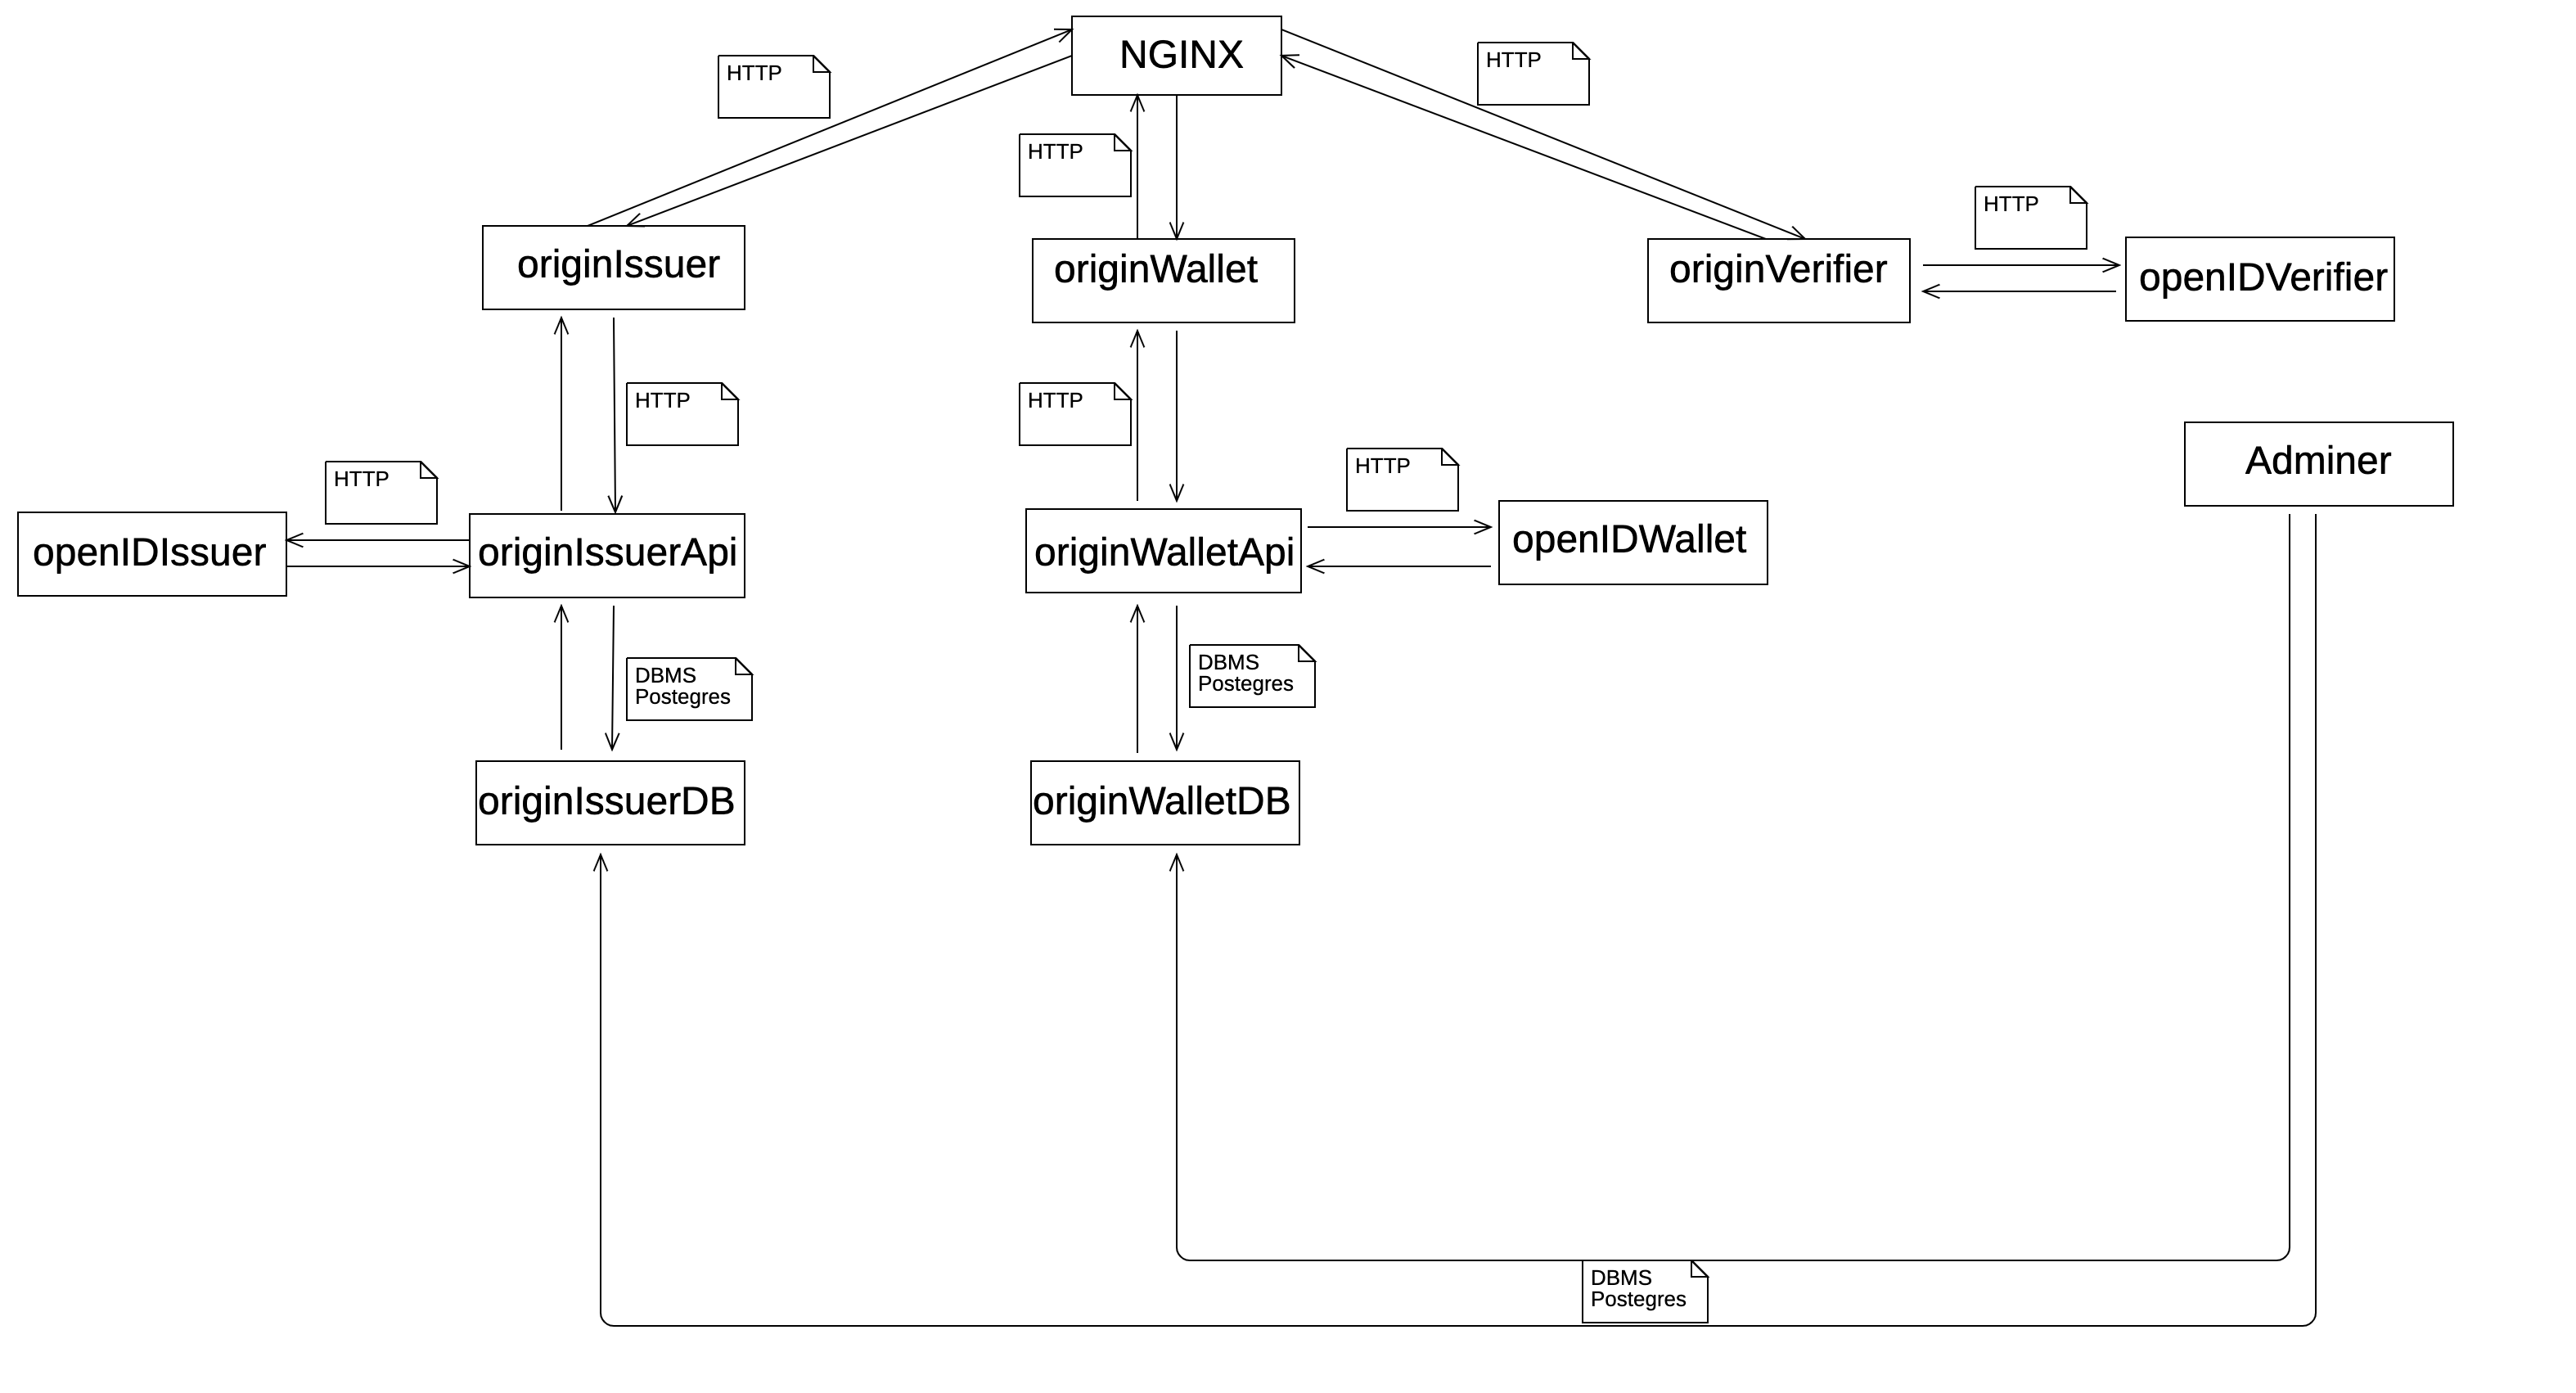
\includegraphics[scale = 0.3]{./res/img/microservizi.png}


\subsubsection{Container \textbf{nginx}}
Lo utilizziamo come server proxy\glo per gestire il reindirezzamento del traffico http tramite domini verso i container interni della rete docker. Alcuni container, nello specifico quelli addibiti allo standard OpenId, utilizzati da noi e sviluppati da WaltId, per funzionare la loro configurazione è basata solo sull'utilizzo di domini. Pertando questo necessita forzatamente l'utilizzo dei precedementemente citati domini per accedere alle funzionalità.  
\subsubsection{Containers dell'\textbf{Issuer}}
\begin{itemize}
    \item \textbf{originIssuerApi:} È la componente di back-end della webapp Issuer che si occupa di gestire le richieste provenienti dal front-end e di comunicare con il database \textit{originIssuerDB} per la memorizzazione dei dati.
    \item \textbf{originIssuer:} È la componete di front-end della webapp Issuer. Essa si interfaccia con l'utente per inviare segnali e ricevere dati dal Back-end \textit{originIssuerApi}. Per la realizzazione del codice è stato adottato il pattern architetturale MVVM (Model-View-ViewModel).
    \item \textbf{originIssuerDB:} È la componente della webapp Issuer che va a eseguire operazioni sul database per la richiesta e la memorizzazione di dati. 
    \item \textbf{openIdIssuer:} È una componente della libreria WaltID per mantenere lo standard openId di comunicazione tra Issuer e le altre webapp, al fine di rispettare le richieste del capitolato.
\end{itemize}
\subsubsection{Containers del \textbf{Wallet}}
\begin{itemize}
    \item \textbf{originWalletApi:} È la componente di back-end della webapp Wallet che si occupa di gestire le richieste provenienti dal front-end e di comunicare con il database \textit{originWalletDB} per la memorizzazione dei dati.
    \item \textbf{originWallet:} È la componete di front-end della webapp Wallet. Essa si interfaccia con l'utente per inviare segnali e ricevere dati dal Back-end \textit{originWalletApi}. Per la realizzazione del codice è stato adottato il pattern architetturale MVVM (Model-View-ViewModel).
    \item \textbf{originWalletDB:} È la componente della webapp Wallet che va a eseguire operazioni sul database per la richiesta e la memorizzazione di dati.
    \item \textbf{openIdWallet:} È una componente della libreria WaltID per mantenere lo standard openId di comunicazione tra Wallet e le altre webapp, al fine di rispettare le richieste del capitolato.
\end{itemize}
\subsubsection{Containers del \textbf{Verifier}}
\begin{itemize}
    \item \textbf{originVerifier:}È la componete di front-end della webapp Verifier. Essa si interfaccia con l'utente per inviare segnali e ricevere dati dal Back-end \textit{originVerfierApi}. Per la realizzazione del codice è stato adottato il pattern architetturale MVVM (Model-View-ViewModel).
    \item \textbf{openIdVerifier:}È una componente della libreria WaltID per mantenere lo standard openId di comunicazione tra Verifier e le altre webapp, al fine di rispettare le richieste del capitolato.
\end{itemize}
\subsubsection{Container \textbf{Adminer}}
È un container che permette agli sviluppatori di gestire i database tramite interfaccia web.

\clearpage

\subsection{Componenti dell'\textbf{Issuer}}

\subsubsection{OriginiIssuerApi (backend)}
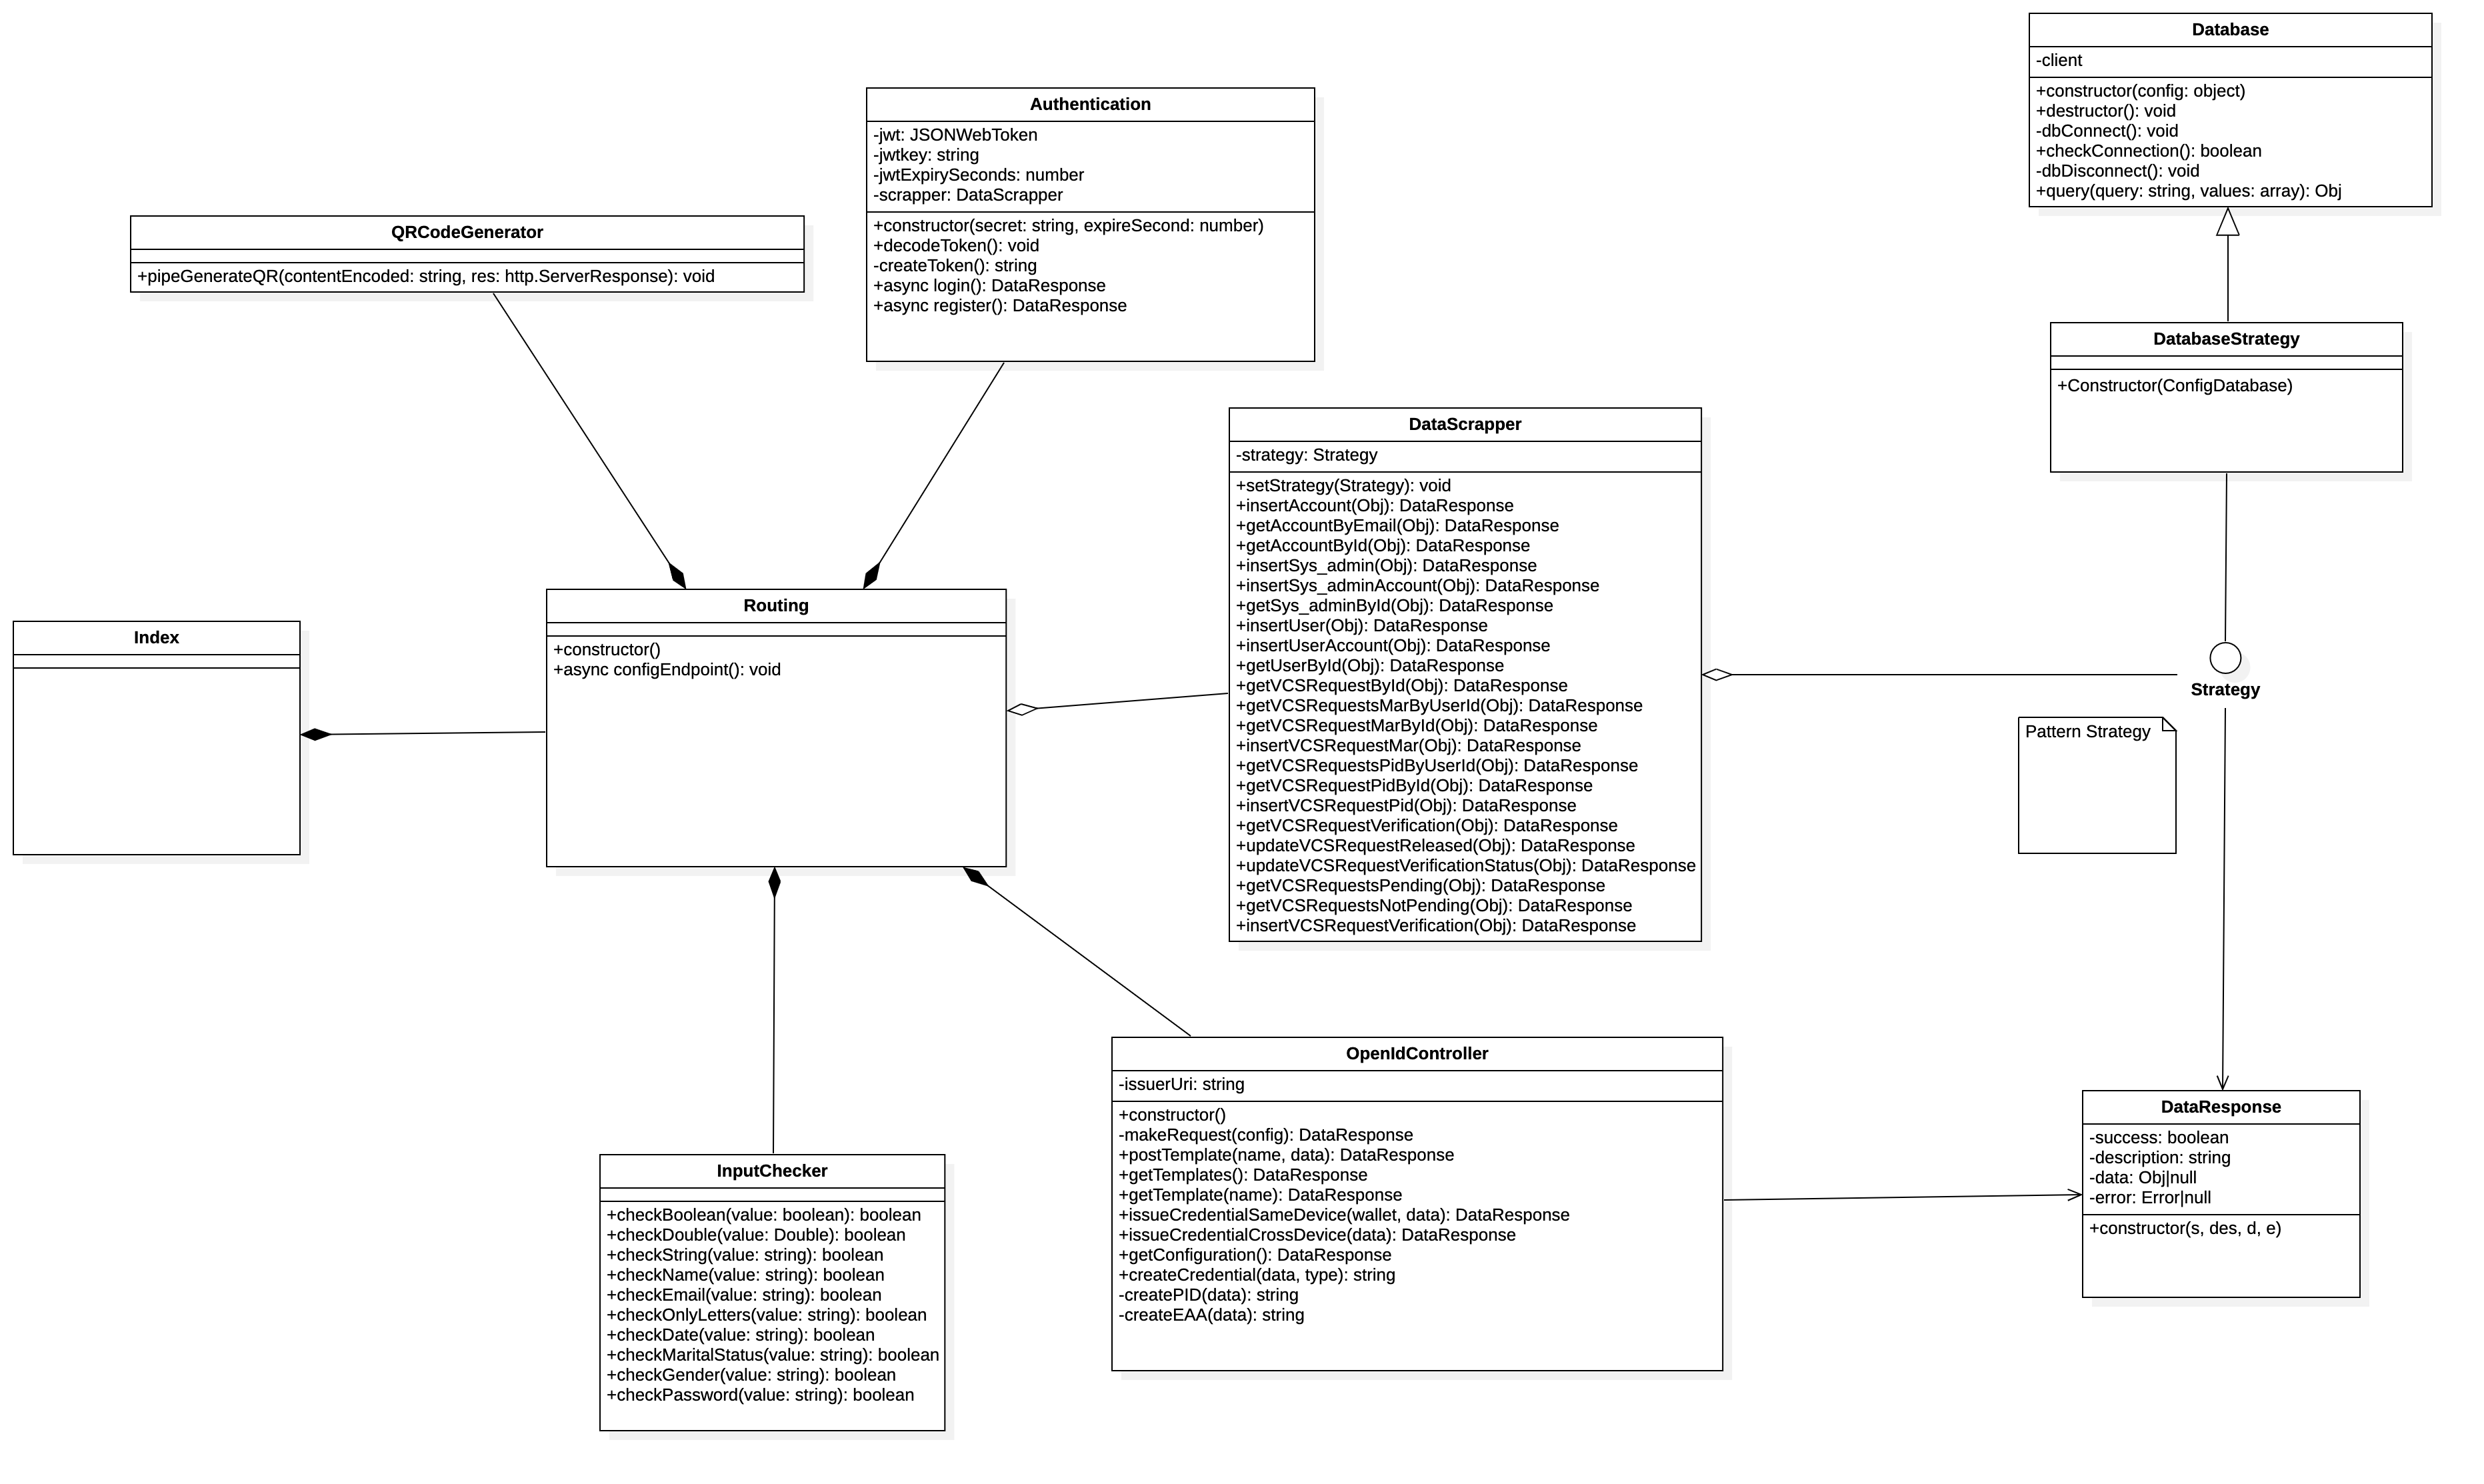
\includegraphics[scale=0.25]{./res/img/backendissuer.png}
\begin{itemize}
    \item \textbf{authentication:}È una classe che si occupa della autenticazione, ovvero: login, registrazione. 
    \item \textbf{datasScrapper:}È un insieme di classi che si occupa di dialogare con il database reperendo e memorizzando i dati da esso. È stato realizzato tramite un insieme di 3 classi che rispettano il pattern strategy. 
    \item \textbf{openid:}È la classe che si occupa di comunicare con il container openIdIssuer. Essendo le chiamate dipendenti strettamente dallo sviluppo della libreria waltId, il gruppo ha preferito far comunicare il front-end non direttamente con la libreria waltId ma dialogare con questo layer intermedio. In questa maniera il backend si occuperà di fare le chiamate con la libreria waltId del container openIdIssuer.
    \item \textbf{DataResponse:}È una classe che si occupa di parametrizzare il tipo di ritorno che il backend fornisce.
    \item \textbf{InputChecker:}Contiene dei metodi necessari per la verifica e la correttezza degli input fatti al backend.
    \item \textbf{QRCodeGenerator:}È una classe fondamentale nel processo di credential issuing. Vi sono 2 modi per generare una credenziale ovvero: cros device e same device. Questa classe si occupa di generare un qrcode senza generare direttamente l'immagine ma dando via risorsa al frontend lo stream dell'immagine del qrcode tramite il metodo \textit{pipeGenerateQR}.
    \item \textbf{Routing:} In questa classe vengono definite 2 funzionalità principali:
     \begin{itemize}
     \item Cors ovvero una funzionalità per limitare l'uso da altri dispositivi. Questa opzione viene configuarata tramite corsOptions specificando gli indirizzi di origine da cui un utilizzatore potrà usare il backend. 
     \item Express è una funzionalità che permette di offrire degli endpoint\glo con cui un altro applicativo potrà fare delle chiamate http. 
     \end{itemize}
    Nel componente vengono configurate le nostre classi precedentemente elencate.
    Inoltre la clsse specifica tutte le chiamate possibili del backend originIssuerApi.
    \item \textbf{index:}Viene creato il routing e il metodo di configurazione degli endpoint.
\end{itemize}

\subsubsection{originIssuer (frontend)} 
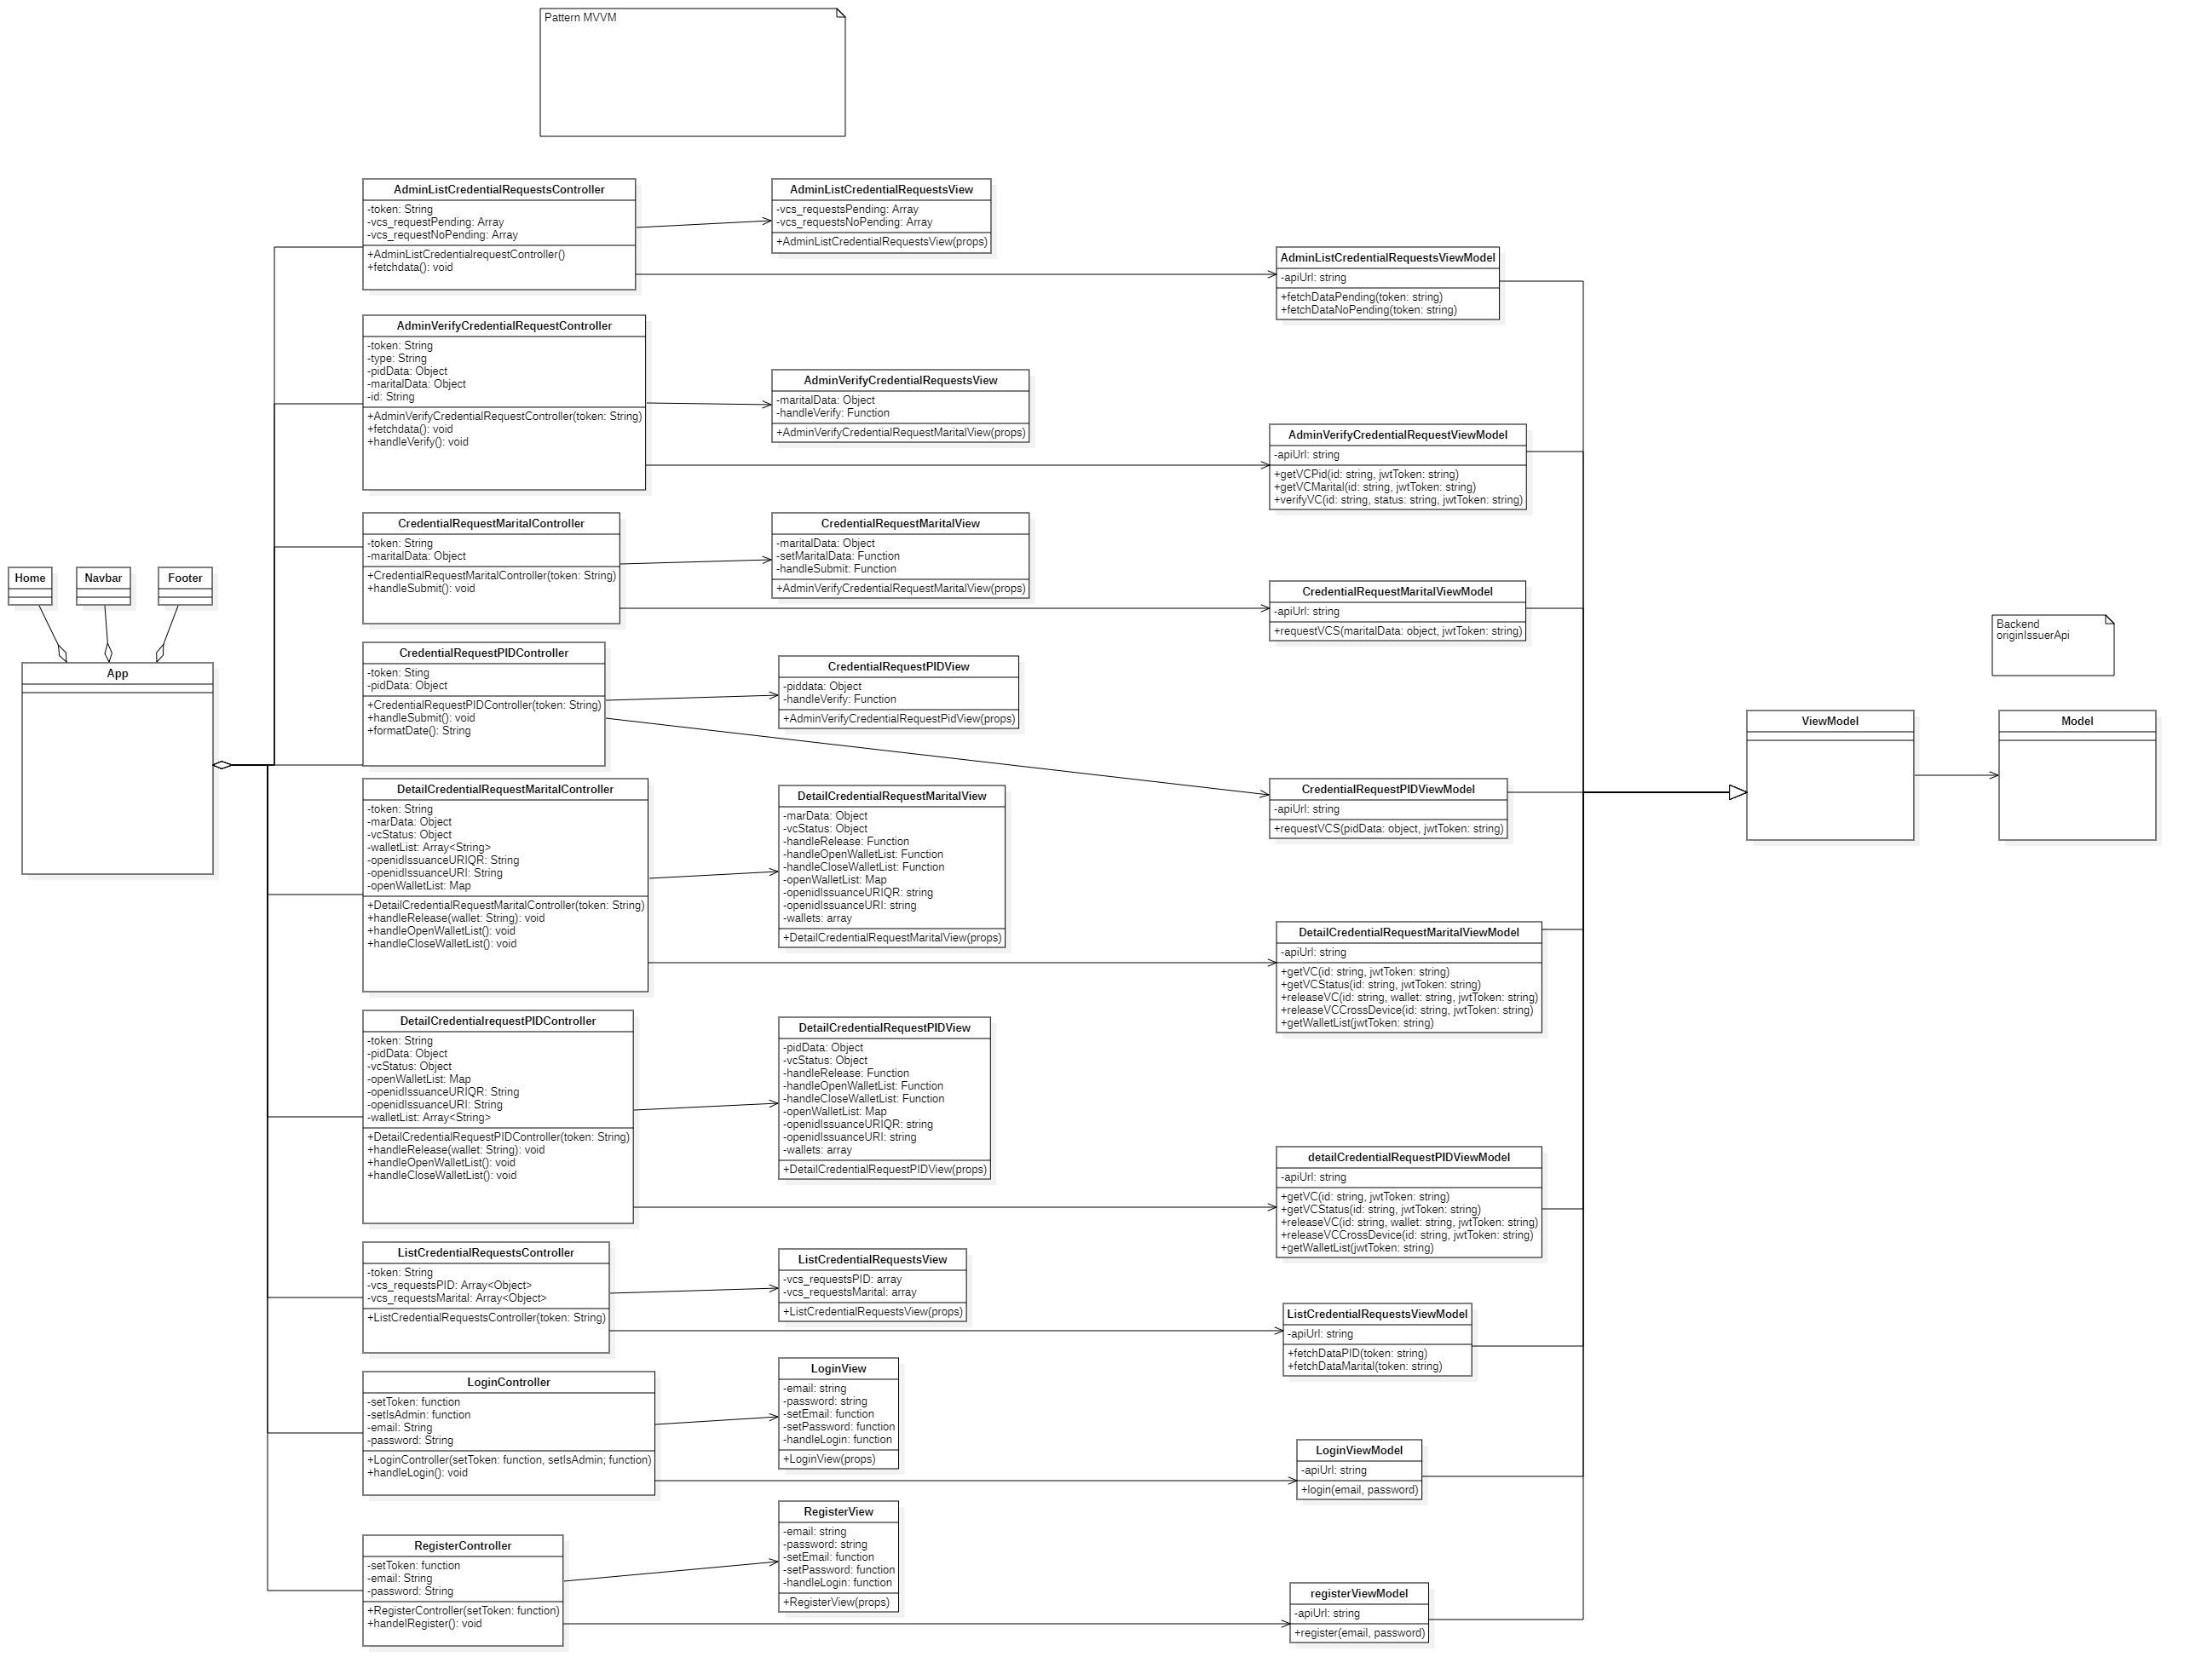
\includegraphics[scale=0.2]{./res/img/frontendissuer.png}
\begin{itemize}
    \item \textbf{components/Navbar:} questa è la componente che definisce la \textit{navbar} dell'applicazione, che differisce dal tipo di utente che è loggato (admin, user, guest).
    \item \textbf{components/useToken:} componente che gestisce la memorizzazione e l'eliminazione del token. Tramite il suo utilizzo si riesce a garantire l'autenticazione del front-end presso il back-end.
    \item \textbf{components/Home:} componente che rappresenta la pagina iniziale dell'applicazione.
    \item \textbf{components/LicenseLable:} componente che gestische i dettagli sulla licenza dell'applicazione.
    \item \textbf{components/Logout:} componente che gestisce il logout dell'utente.
\end{itemize}

Ogni seguente componente è composta da 3 parti: \textit{controller}, \textit{viewmodel} e \textit{view}. Il controller crea la corrispondente
viewModel e view. Il controller si occupa di gestire gli eventi provenienti dalla view e di aggiornare la viewModel, che a sua volta aggiorna 
il model presente nel back-end. La view si occupa di mostrare i dati presenti nella viewModel e di gestire gli eventi provenienti dall'utente.

\begin{itemize}
    \item \textbf{Login:} questa è la componente che gestisce la pagina di login dell'applicazione. 
    \item \textbf{Register:} questa è la componente che gestisce la pagina di registrazione dell'applicazione.
    \item \textbf{CredentialRequestPID:} questa è la componente che gestisce la pagina di richiesta di una credenziale PID.
    \item \textbf{CredentialRequestMarital:} questa è la componente che gestisce la pagina di richiesta di una credenziale Marital.
    \item \textbf{ListCredentialReqauest:} questa è la componente che gestisce la pagina di visualizzazione delle richieste di credenziali. Si viene reindirizzati
    a questa pagina dopo aver fatto richiesta di una credenziale.
    \item \textbf{DetailCredentialRequestPID:} questa è la componente che gestisce la pagina di dettaglio di una richiesta di credenziale PID.
    \item \textbf{DetailCredentialRequestMarital:} questa è la componente che gestisce la pagina di dettaglio di una richiesta di credenziale Marital.
    \item \textbf{AdminListCredentialRequest:} questa è la componente che gestisce la pagina di visualizzazione delle richieste di credenziali da parte degli admin.
    In essa sono presenti due liste di richieste: quelle da approvare e quelle già approvate.
    \item \textbf{AdminVerifyCredentialRequest:} questa è la componente che gestisce la pagina di dettaglio di una richiesta di credenziale da parte degli admin.
\end{itemize}

\subsubsection{originIssuerDB (database):}
    \begin{center}
        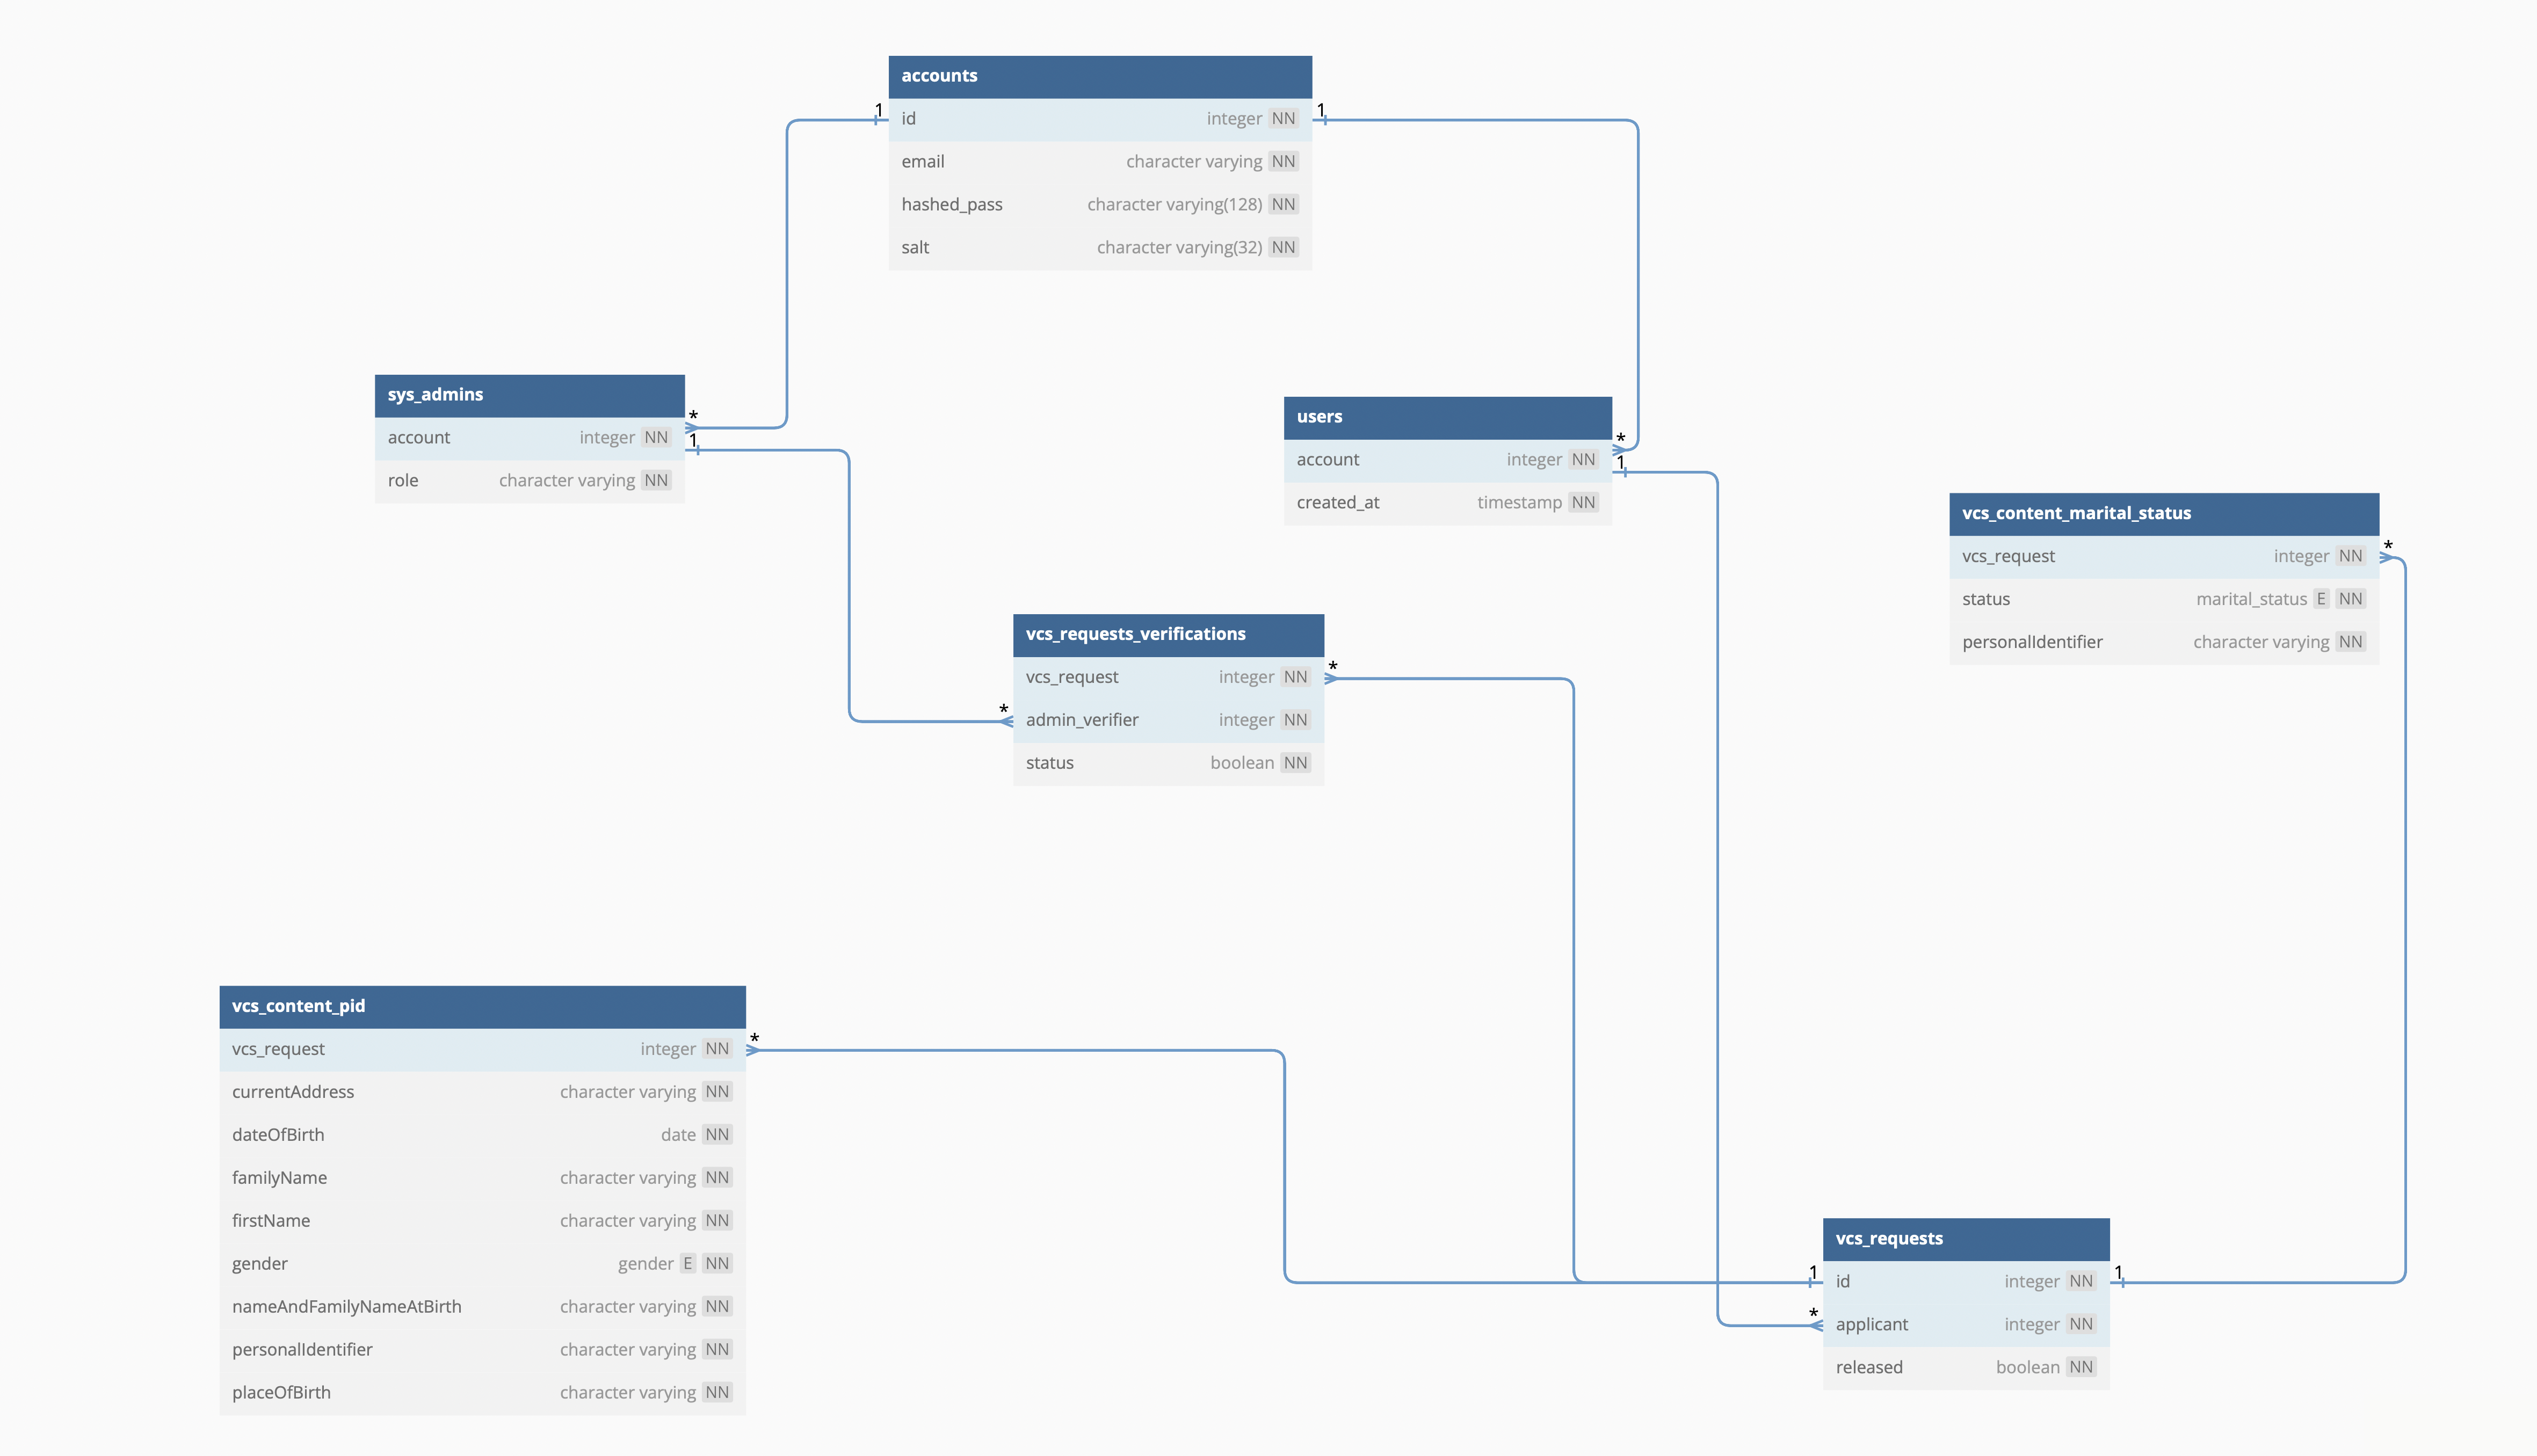
\includegraphics[scale = 0.2]{./res/img/issuerdb.png}
      \end{center}
    L'immagine sopra riportata descrive il database "issuerdb" implementato mediante un diagramma logico.\\
    Issuerdb è stato pensato per gestire e conservare le informazioni legate agli utenti, alle richieste di certificati digitali (VCS requests) e alle verifiche dei certificati stessi.
    Per quanto richiesto dal capitolato, e per rispettare la logica dietro tutto il meccanismo dell'Issuer, si distinguono 2 tipi diversi di account: gli account "sys\_admins" e gli account "users".\\
    \begin{itemize}
    \item "sys\_admins" sono gli account utilizzati dagli amministratori di sistema, cioè quelle entità che si occupano di approvare (o meglio, verificare) le richieste degli "users" (VCS requests).\\
    \item "users", invece, sono gli account utilizzati dai semplici utilizzatori del servizio. Si occupano semplicemente di effettuare delle richieste di certificati di loro interesse alle entità che si occupano di verificare i certificati.\\
    \end{itemize}
    Il contenuto della richiesta approvata e rilasciata può essere di 2 tipi soltanto: un "vcs\_content\_marital\_status" (contenuto riferito allo stato di matrimonio di un utente) o un "vcs\_content\_pid" (contenuto riferito ad un documento PID di un utente).\\

\subsection{Componenti del \textbf{Wallet}}

\subsubsection{OriginWalletApi (backend)}
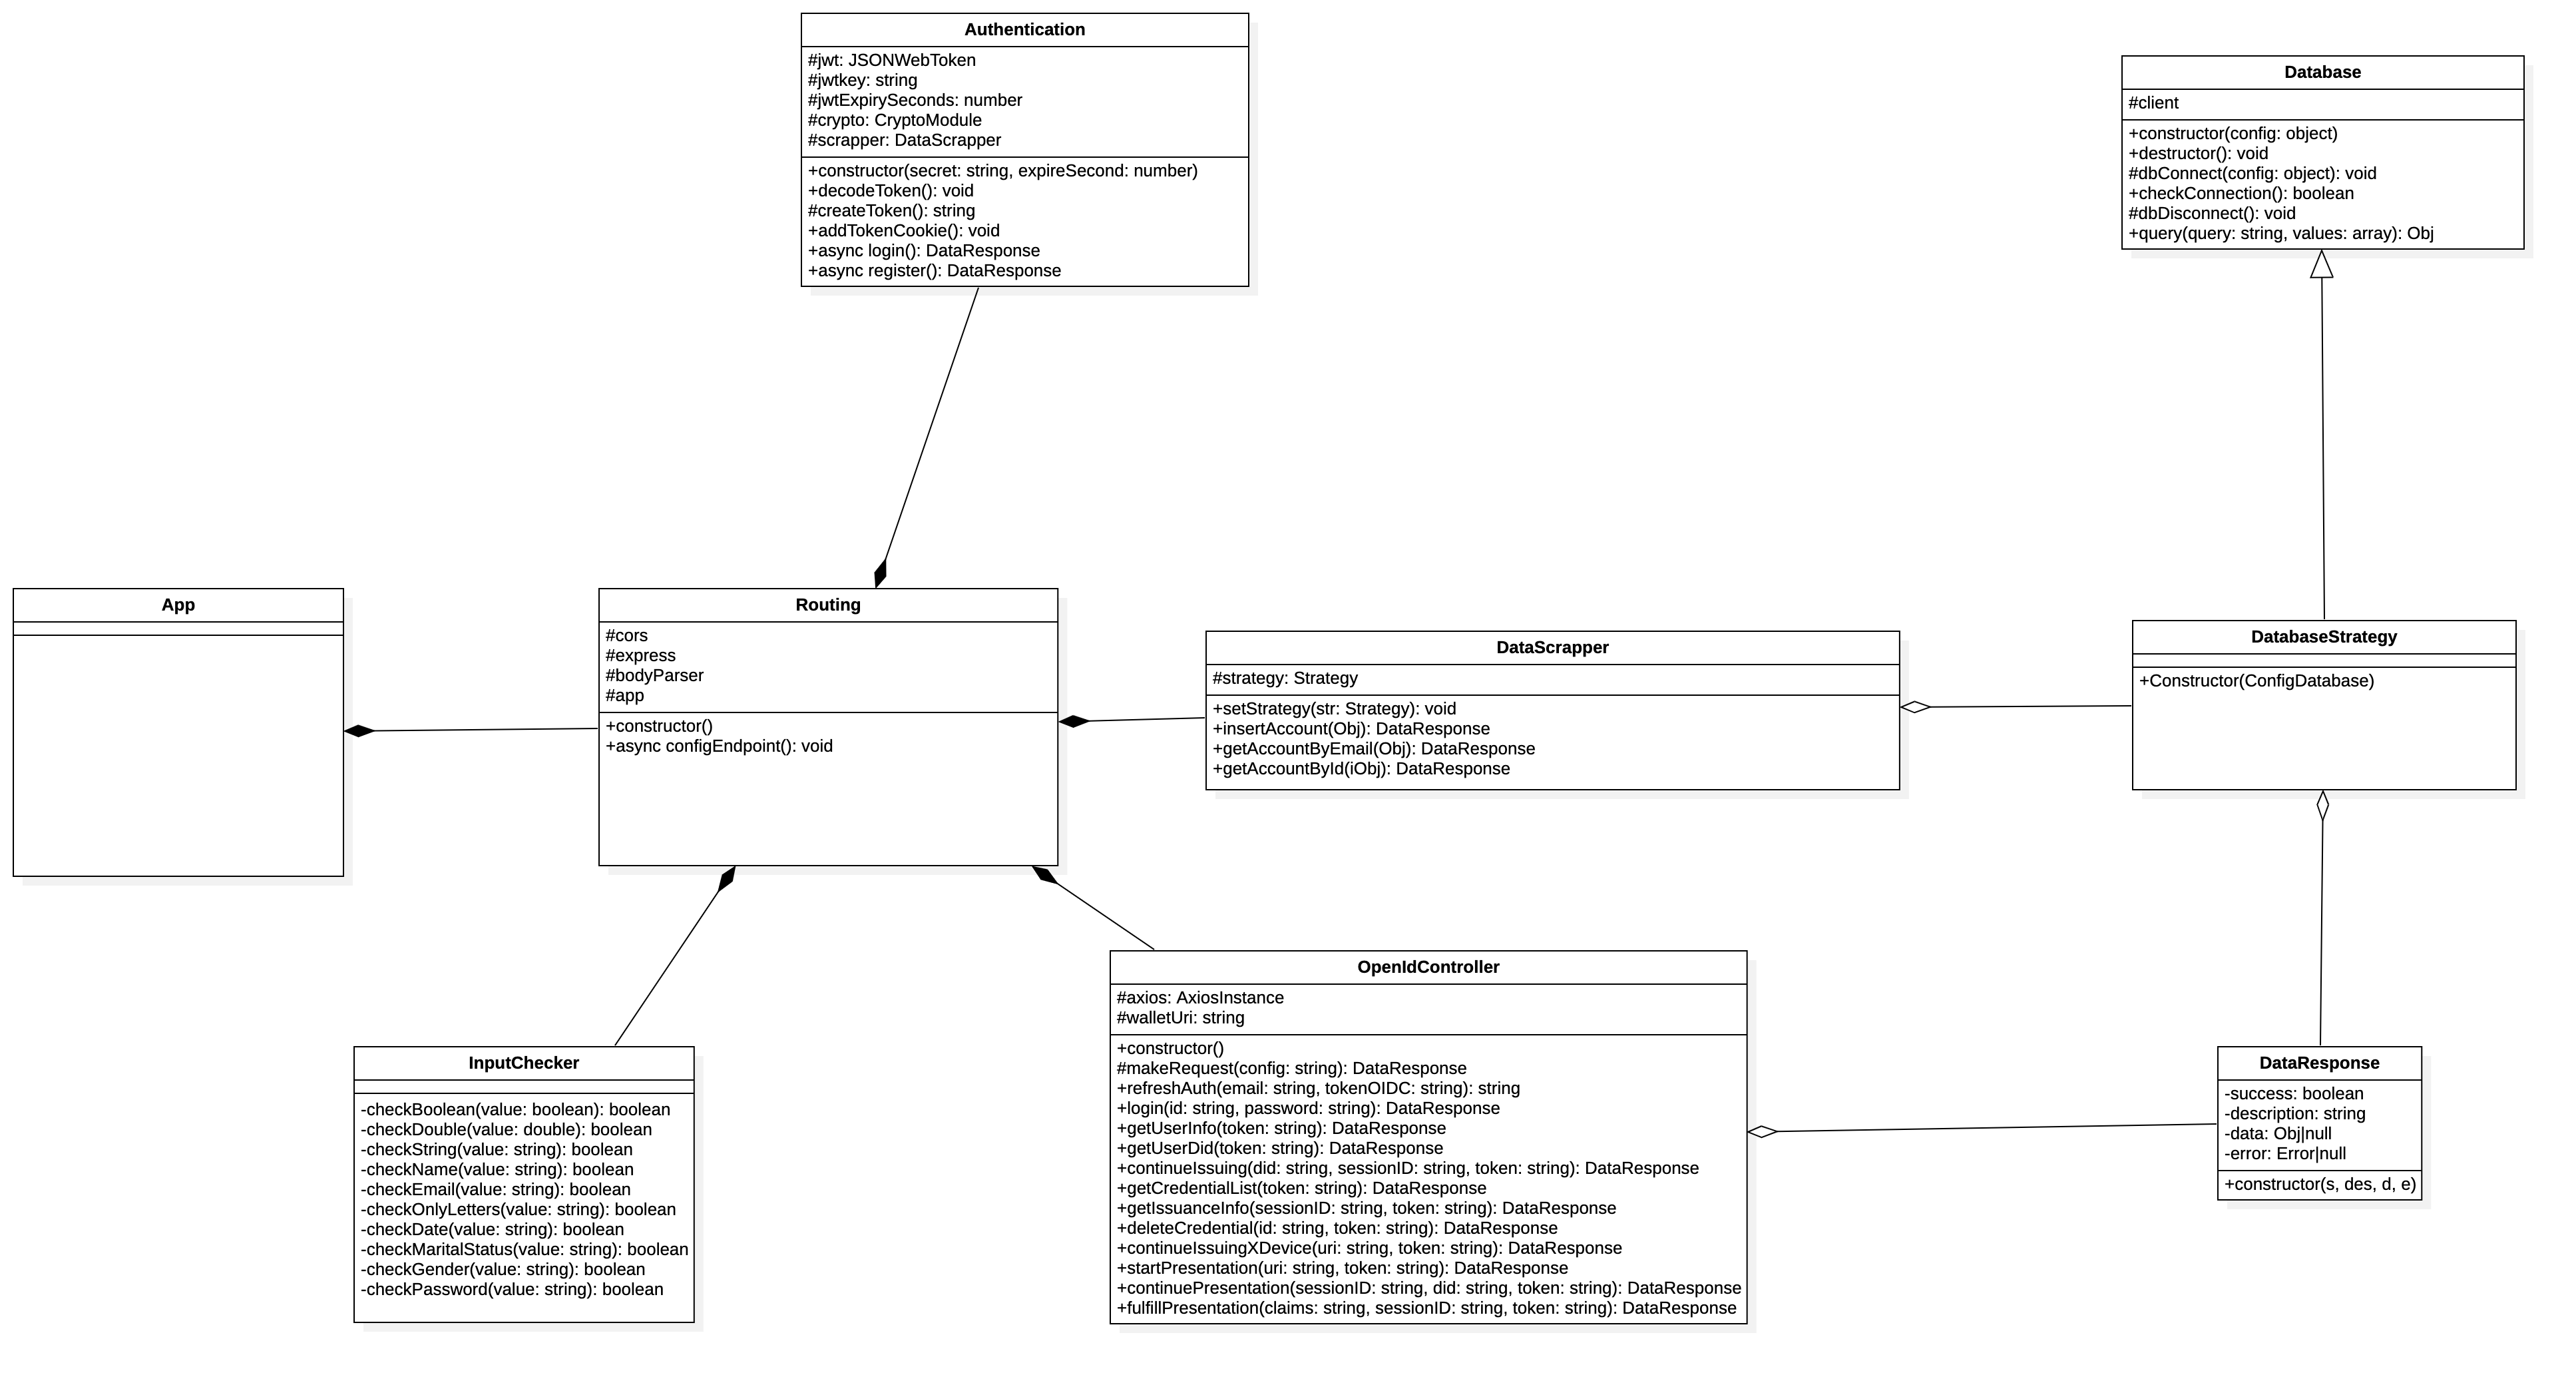
\includegraphics[scale=0.25]{./res/img/backendwallet.png}
\begin{itemize}
    \item \textbf{authentication:}È una classe che si occupa della autenticazione, ovvero: login, registrazione. 
    \item \textbf{datasScrapper:}È un insieme di classi che si occupa di dialogare con il database reperendo e memorizzando i dati da esso. È stato realizzato tramite un insieme di 3 classi che rispettano il pattern strategy. Essendo il database del Wallet irrisorio si potrebbe usare un ulteriore strategia, memorizzando i dati su un file XML o JSON. Questo poichè la struttura dei dati e la complessità è semplice e senza relazioni particolari.
    \item \textbf{openid:}È la classe che si occupa di comunicare con il container openIdWallet. Essendo le chiamate dipendenti strettamente dallo sviluppo della libreria waltId, il gruppo ha preferito far comunicare il front-end non direttamente con la libreria waltId ma dialogare con questo layer intermedio. In questa maniera il backend si occuperà di fare le chiamate con la libreria waltId del container openIdWallet.
    \item \textbf{DataResponse:}È una classe che si occupa di parametrizzare il tipo di ritorno che il backend fornisce.
    \item \textbf{InputChecker:}Contiene dei metodi necessari per la verifica e la correttezza degli input fatti al backend.
    \item \textbf{Routing:} In questa classe vengono definite 2 funzionalità principali:
    \begin{itemize}
    \item Cors ovvero una funzionalità per limitare l'uso da altri dispositivi. Questa opzione viene configuarata tramite corsOptions specificando gli indirizzi di origine da cui un utilizzatore potrà usare il backend. 
    \item Express è una funzionalità che permette di offrire degli endpoint con cui un altro applicativo potrà fare delle chiamate http. 
    \end{itemize}
    Nel componente vengono configurate le nostre classi precedentemente elencate.
    Inoltre la clsse specifica tutte le chiamate possibili del backend originIssuerApi.
\end{itemize}

\subsubsection{originWallet (frontend)}
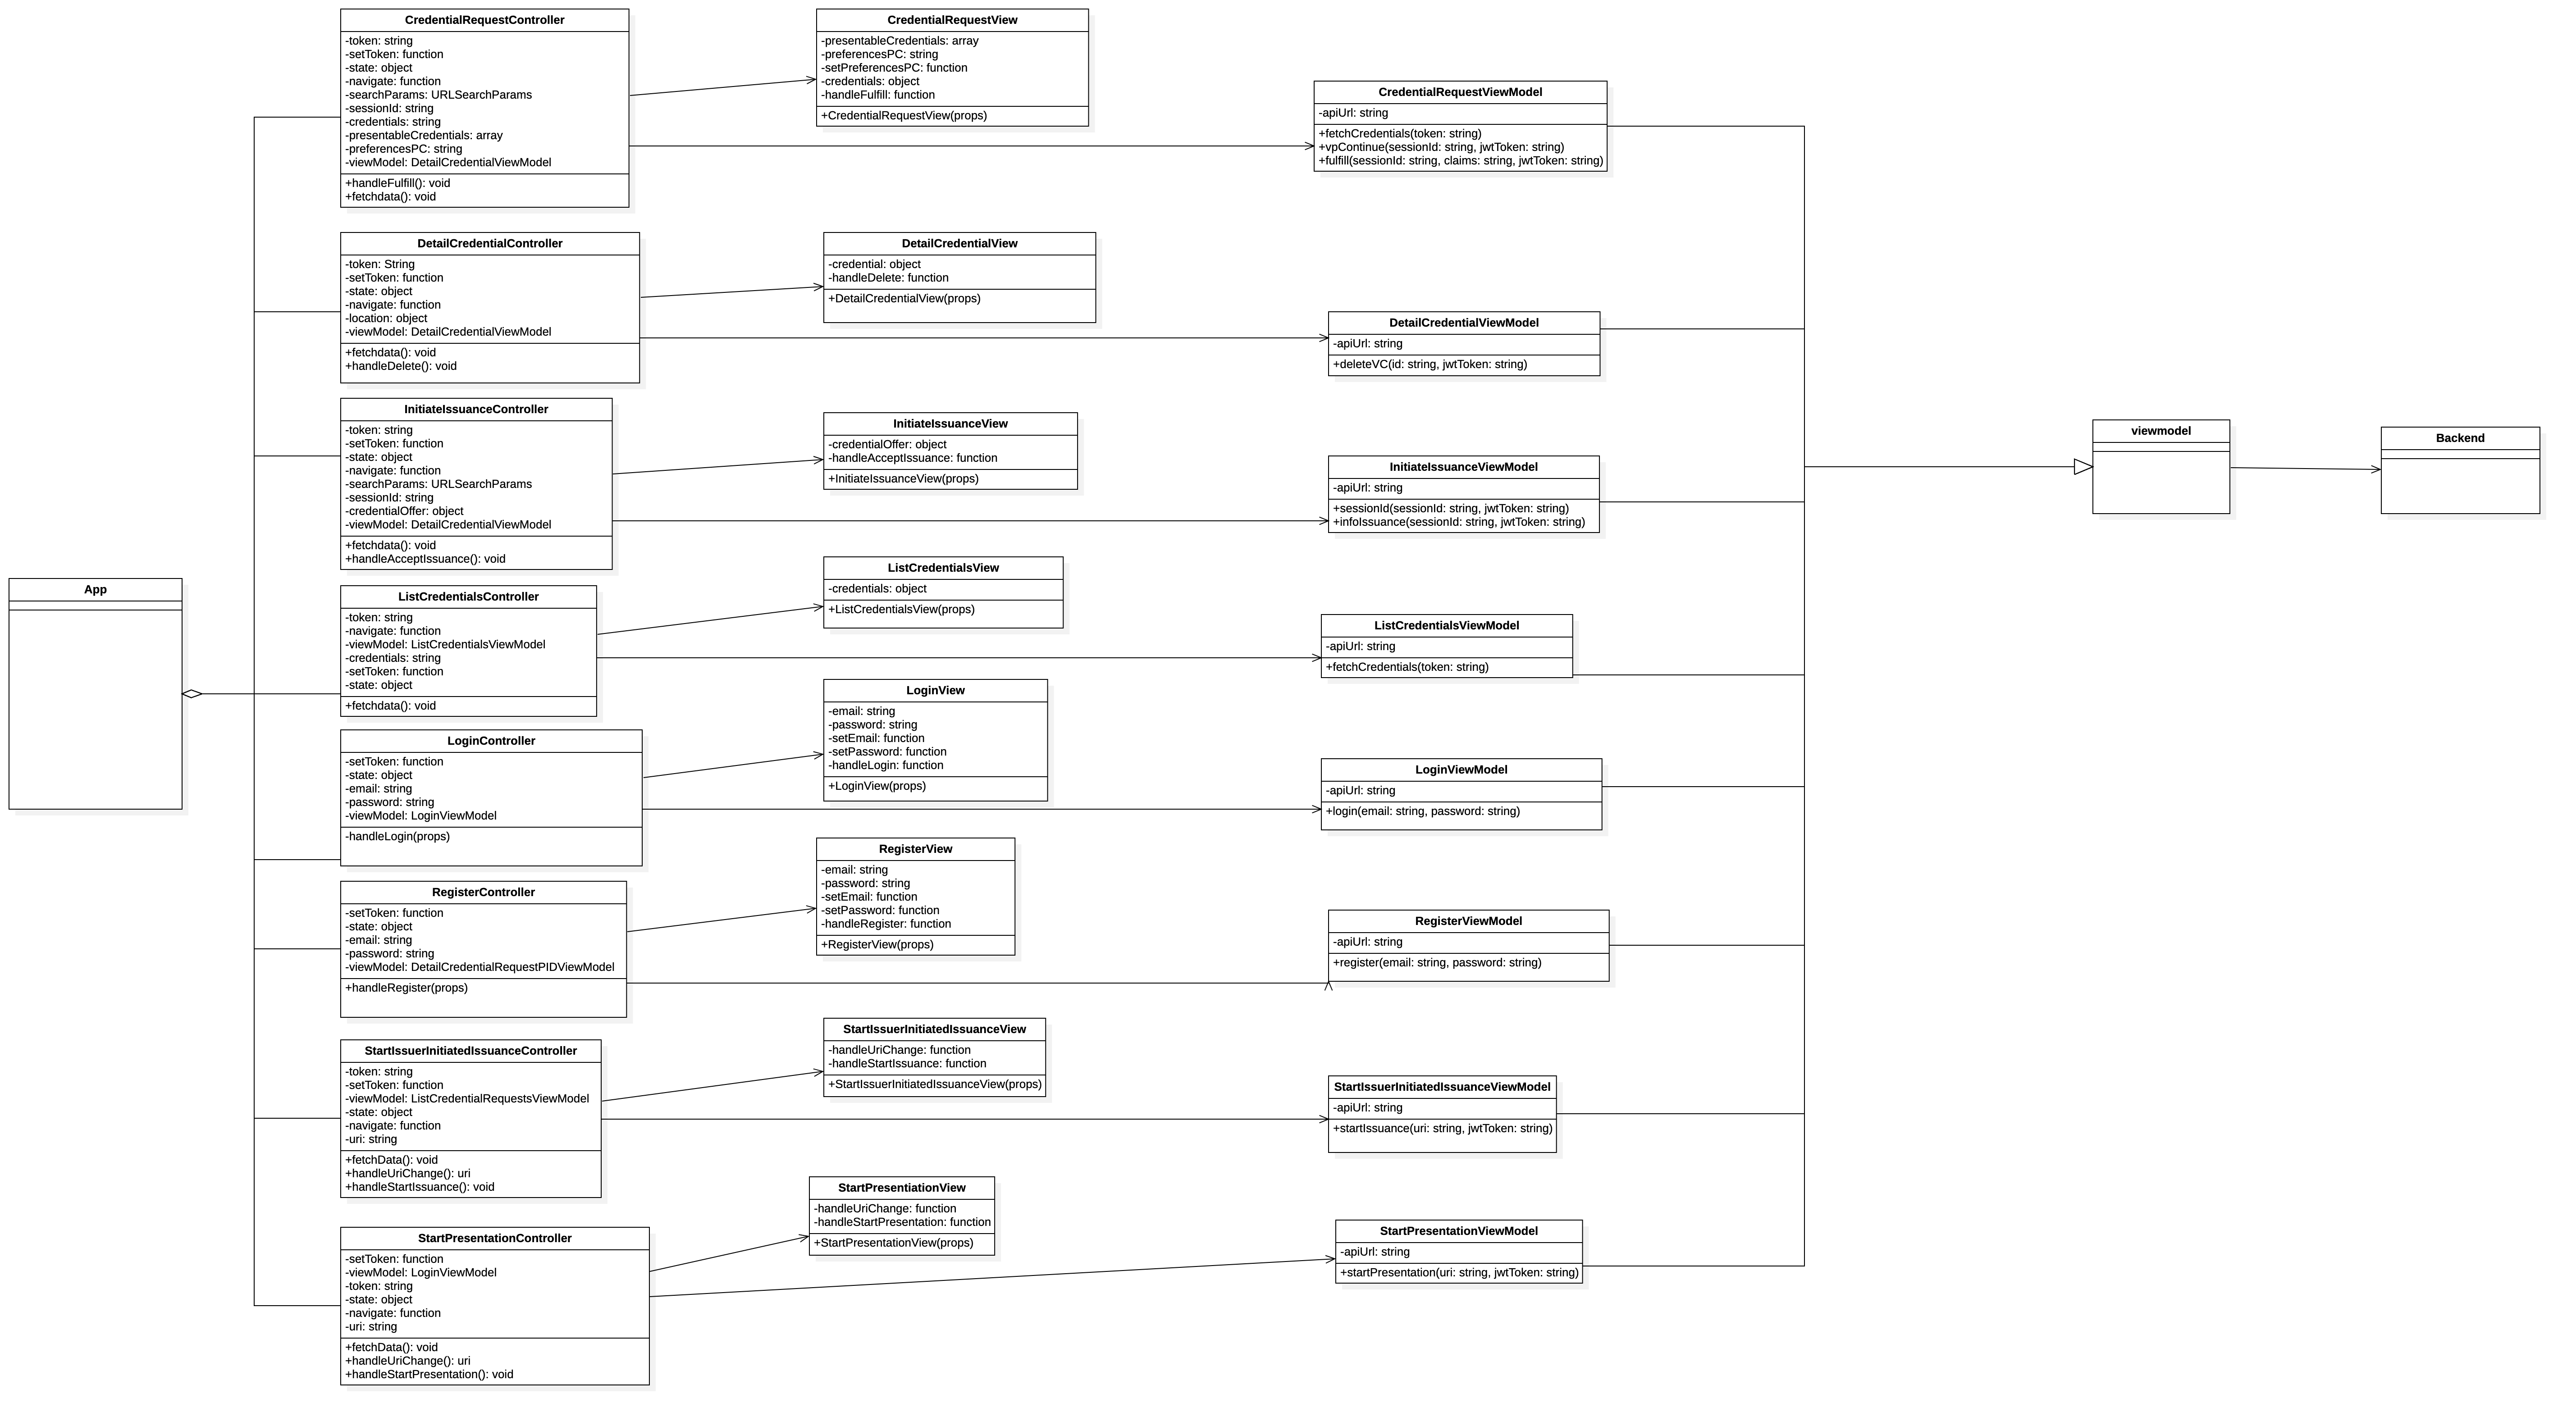
\includegraphics[scale=0.2]{./res/img/frontendwallet.png}
\begin{itemize}
    \item \textbf{App:} questa è la pagina iniziale dell'applicazione, dove viene definito il \textit{routing} delle pagine.
    \item \textbf{components/Navbar:} questa è la componente che definisce la \textit{navbar} dell'applicazione, che differisce dal tipo di utente che è loggato (user, guest).
    \item \textbf{components/useToken:} componente che gestisce la memorizzazione e l'eliminazione del token. Tramite il suo utilizzo si riesce a garantire l'autenticazione del front-end presso il back-end.
    \item \textbf{components/Home:} componente che rappresenta la pagina iniziale dell'applicazione.
    \item \textbf{components/LicenseLable:} componente che gestische i dettagli sulla licenza dell'applicazione.
    \item \textbf{components/Logout:} componente che gestisce il logout dell'utente.  
    \item \textbf{pageState:} componente che gestisce il dialogo ed il reindirizzamento tra le applicazioni. Questa componente memorizza lo stato in cui si trova il \textit{wallet} prima di un reindirizzamento e lo riprende dopo che questo è terminato.
\end{itemize}

Ogni seguente componente è composta da 3 parti: \textit{controller}, \textit{viewmodel} e \textit{view}. Il controller crea la corrispondente
viewModel e view. Il controller si occupa di gestire gli eventi provenienti dalla view e di aggiornare la viewModel, che a sua volta aggiorna 
il model presente nel back-end. La view si occupa di mostrare i dati presenti nella viewModel e di gestire gli eventi provenienti dall'utente.

\begin{itemize}      
    \item \textbf{Login:} questa è la componente che gestisce la pagina di login dell'applicazione. 
    \item \textbf{Register:} questa è la componente che gestisce la pagina di registrazione dell'applicazione.
    \item \textbf{ViewModel:} componente che si occupa del collegamento con il back-end, ha quindi un riferimento al \textit{model}. È unico per tutta l'applicazione.
    \item \textbf{ListCredential:} componente che si occupa di mostrare la lista delle credenziali dell'utente presenti nel \textit{Wallet}. Da qui si può andare nel dettaglio di una singola credenziale.
    \item \textbf{DetailCredential:} componente che si occupa di mostrare i dettagli di una credenziale presente nel \textit{Wallet}. Da qui si può eliminare una credenziale.\\
    \\NB. Le seguenti componenti hanno nomi controintuitivi ma sono imposti dallo standard \textit{openID}.
    \item \textbf{InitiateIssuance:} componete che si  occupa dell'accettazione di una richiesta di credenziale da parte di un \textit{Issuer} e vengo reindirizzato alla pagina \textit{ListCredential}.
    \item \textbf{CredentialRequest:} componente che si occupa del re indirizzamento di una richiesta di presentazione di una credenziale parte del \textit{Verifier}. 
    \item \textbf{StartIssuerInitiatedIssuance:} componente necessaria per il \textit{credential issuing} cross-device, quindi attraverso URI openID.
    \item \textbf{StartPresentation:} componente necessaria per la \textit{verifiable presentation} cross-device, quindi fare il fullfill di una presentazione attraverso URI openID.
\end{itemize}

\subsubsection{originWalletDB (database):}
     \begin{center}
        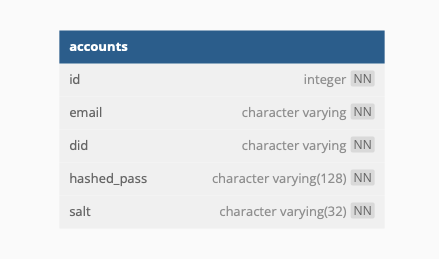
\includegraphics[scale = 0.6]{./res/img/walletdb.png}
      \end{center}
    
    L’immagine sopra riportata descrive il database “walletdb” implementato mediante un diagramma logico.
    Walletdb è stato pensato per gestire e conservare (fare lo “storing”) le informazioni legate alle credenziali degli utenti, come espresso da capitolato.\\
    

\subsection{Componenti del \textbf{Verifier}}
\subsubsection{originVerifier (frontend)}
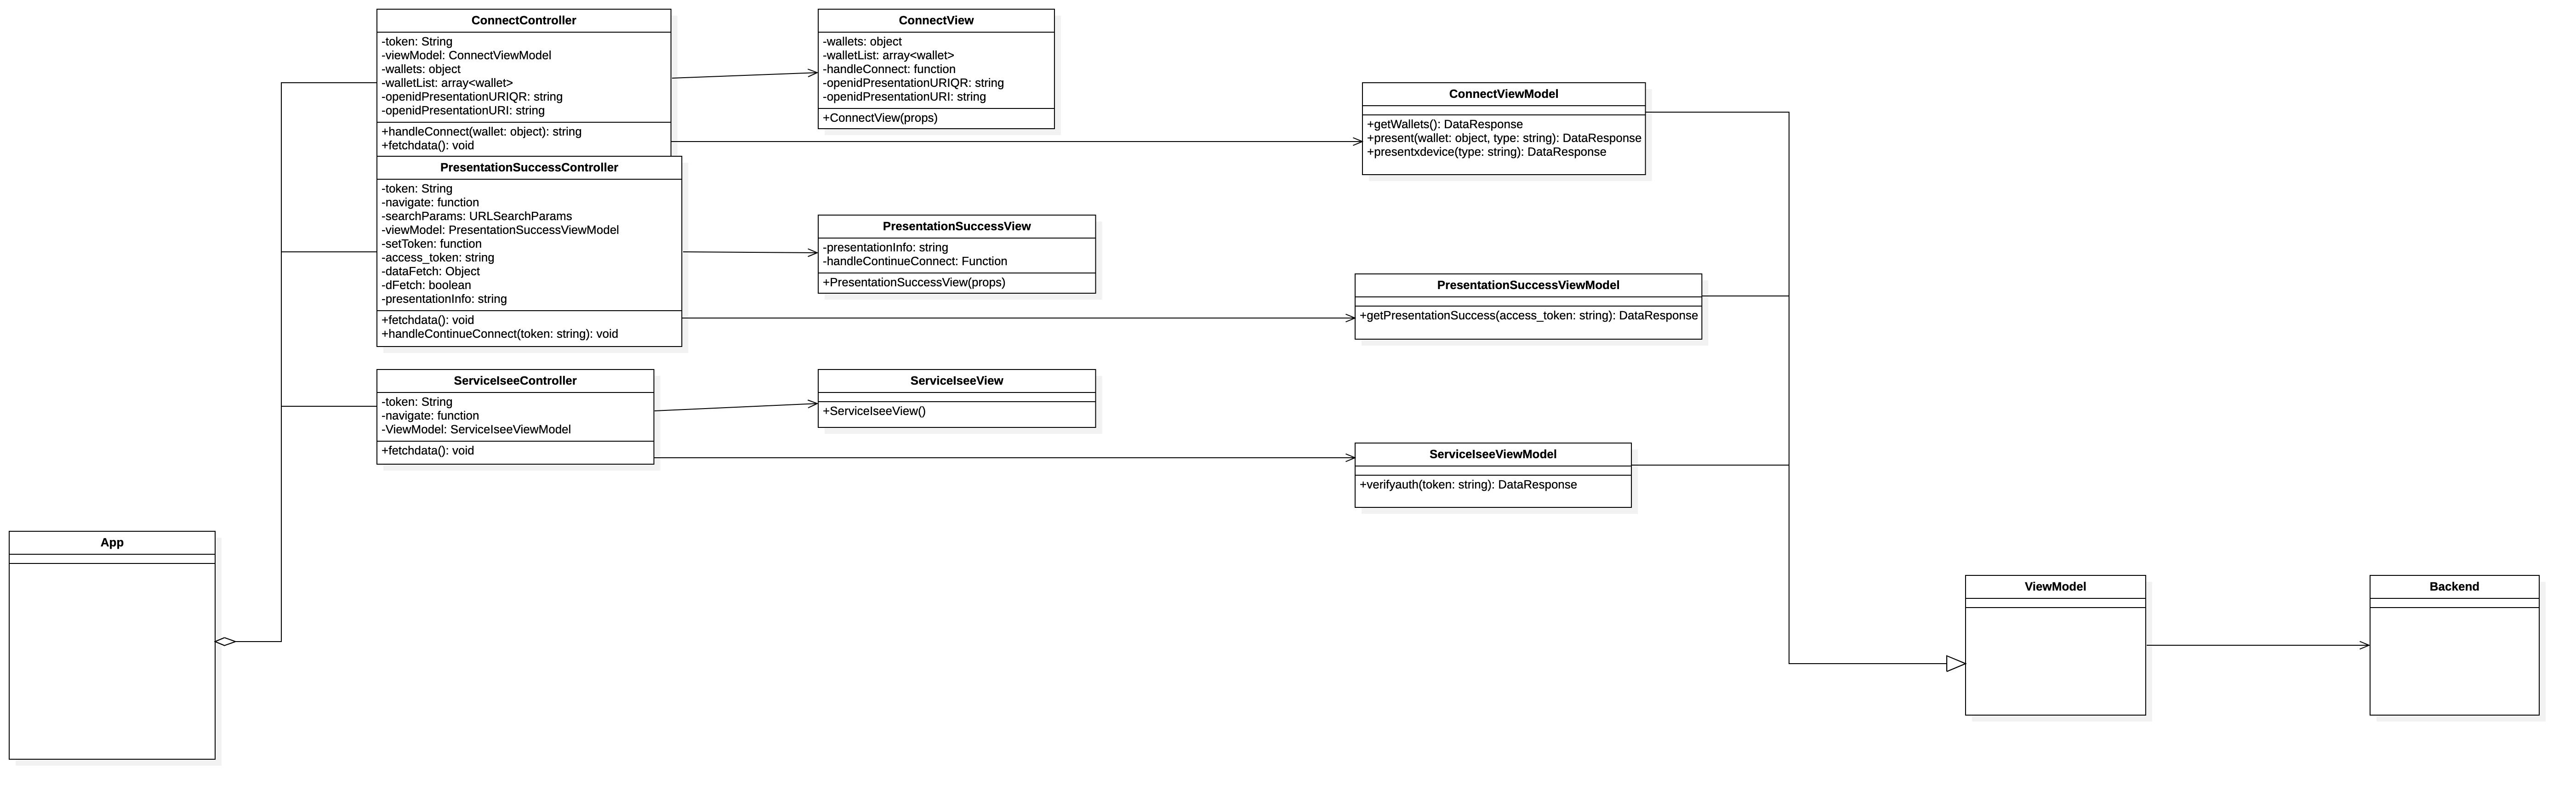
\includegraphics[scale=0.22]{./res/img/frontendverifier.png}
\begin{itemize}
    \item \textbf{App:} questa è la pagina iniziale dell'applicazione, dove viene definito il \textit{routing} delle pagine.
    \item \textbf{components/Navbar:} questa è la componente che definisce la \textit{navbar} dell'applicazione, che differisce dal tipo di utente che è loggato.
    \item \textbf{components/useToken:} componente che gestisce la memorizzazione e l'eliminazione del token. Tramite il suo utilizzo si riesce a garantire l'autenticazione del front-end presso il back-end.
    \item \textbf{components/Home:} componente che rappresenta la pagina iniziale dell'applicazione.
    \item \textbf{components/LicenseLable:} componente che gestische i dettagli sulla licenza dell'applicazione.
    \item \textbf{components/Logout:} componente che gestisce il logout dell'utente.  
\end{itemize}

Ogni seguente componente è composta da 3 parti: \textit{controller}, \textit{viewmodel} e \textit{view}. Il controller crea la corrispondente
viewModel e view. Il controller si occupa di gestire gli eventi provenienti dalla view e di aggiornare la viewModel, che a sua volta aggiorna 
il model presente nel back-end. La view si occupa di mostrare i dati presenti nella viewModel e di gestire gli eventi provenienti dall'utente.

\begin{itemize}
    \item Connect: componente necessaria per effettuare la connesione e presentare una credenziale di tipo PID al \textit{Verifier} attraverso il proprio \textit{Wallet}.
    \item PresentationSuccess: componente che si occupa di mostrare il successo della presentazione di una credenziale.
    \item ServiceIsee: servizio offerto dal \textit{Verifier} che simula la richiesta di un ISEE, per acceder a questo componente si è vincolati all'utilizzo di un token di autorizzazione rilasciato dal componente openID e rilasciato solo in nel caso la procedura di verifiable presentation è completata con successo. 
\end{itemize}

\subsection{Design pattern}
\subsubsection{Strategy}
Il Pattern Strategy è un design pattern comportamentale che consente ad un oggetto client di scegliere un algoritmo specifico tra una serie di diversia algoritmi senza dover necessariamente modificare il codice sorgente. Questo favorisce la modularità, la flessibilità del codice e l'incapsulamento. 
Esso è stato utilizzato per la componente del Wallet e dell'Issuer. Essendo che entrambe hanno la necessità, in quanto web application, di collegarsi al backend. Quest'ultimo deve memorizzare, richiedere e visualizzare i dati in un database. Il gruppo ha deciso di adottare tale pattern data la possibilità in futuro di cambiare sistema di dbms o struttura di contenimento di dati (XML o JSON) cambiando soltanto algoritmo senza dover cambiare il codice sorgente per intero. 
Questo è stato possibile attraverso l'utilizzo di 3 classi: \textit{dataScapper} essendo l'interfaccia principale con la quale la web application interagiasce, tramite il metodo setStrategy è stato utilizzata la strategia \textit{DatabaseStrategy}. Quest'ultima è una strategia di reperimento dei dati specifici, applicata per una tipologia specifica di database; ereditata dalla classe \textit{Database}. 
Il pattern utilizzato si discosta da quello imparato durante il corso poichè il linquaggio di programmazione Javascript non implementa l'ereditarietà nelle classi. Per sopperire a tale mancanza è stata usata la relazione \textit{has-a}.
Nel Nostro caso ad esempio essendo il database di Wallet semplice e con nessuna relazione è possibile in futuro applicare una strategia JSONStrategy al posto di DatabaseStrategy.

\subsubsection{Il pattern architetturale Model-View-ViewModel}
È stato utilizzato per separare la parte di business logic dell'applicazione da quella della'ui per rendere più manutenibile il codice e per mantenere una gestione più chiara dei dati e dell'interfaccia utente. \\
In particolare abbiamo applicato il pattern secondo la seguente struttura : 

\begin{center}
    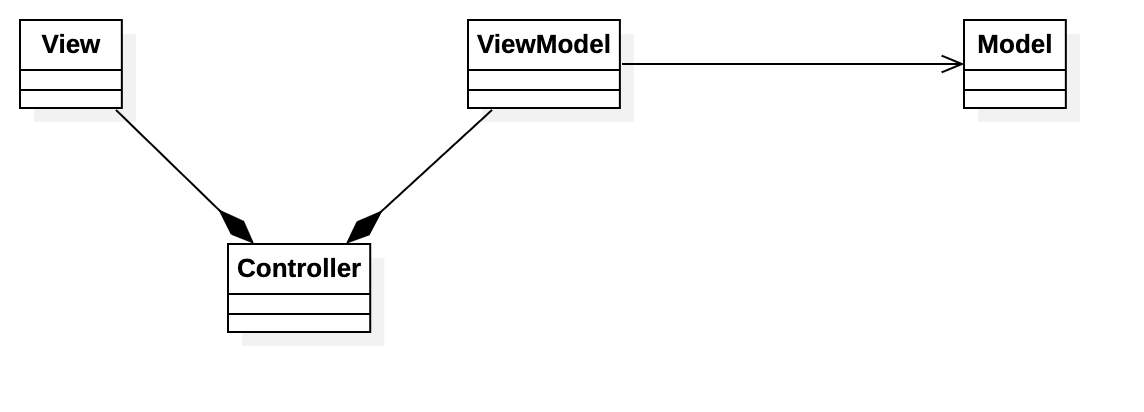
\includegraphics[scale = 0.4]{./res/img/MVVM.png}
  \end{center}
  
Introducendo la componente controller all'interno del pattern abbiamo un interazione in più tra la view e il ViewModel. Questo ci permette di:
\begin{itemize}
    \item Riusciamo a gestire meglio gli handler, ovvero le funzioni chiamate;
    \item riusciamo meglio a gestire gli eventi;
    \item riusciamo meglio a gestire i dati ed elaborarli.
\end{itemize}

Nello specifico quset'ultimo punto era necessario poichè non dovevamo soltanto mostrare dei dati presi direttamnete dal database. In questa maniera abbiamo usato il controller come component di react. Questa struttura è stata adottata per tutte e 3 le web application. 